\chapter{Conclusão}

    Visando solucionar a demanda da empresa
    Rio Branco Alimentos SA/ Fábrica de Rações de Patrocínio
    da melhor forma possível cumpri-se todos os requisitos 
    por eles exigidos na descrição da demanda no Portal Saga SENAI
    foi idealizado esse projeto para de forma simples e eficaz 
    sanar as dores de nosso cliente.

    Para solucionar a demanda serão instalados sensores de 
    temperatura em cada freezer
    e assim poder informar os usuários sobre a temperatura
    interna das vacinas e emitir um alerta caso a temperatura
    saia de uma faixa predeterminada, normalmente de 2 a 8 ºC.

    Com o propósito de criar um histórico com as variações de 
    temperatura de cada freezer os dados de cada sensor de 
    temperatura serão transmitidos e guardados em um 
    banco de dados que poderá ser consultado a qualquer momento
    pelos usuários, também será possível visualizar a temperatura
    em tempo real de cada freezer e receber alerta e notificações
    caso a temperatura saia do nível esperado.

    Com esse projeto escrito pelos autores 
    será possível evitar várias perdas de vacinas por 
    falta de gerenciamento da temperatura dos freezeres
    em que as mesmas são guardadas, além de gerar maior valor 
    agregado ao processo e ao produto, garantindo 
    a qualidade e a confiabilidade das vacinas.

    \begin{figure}
        \caption{Canvas}
        \centering
        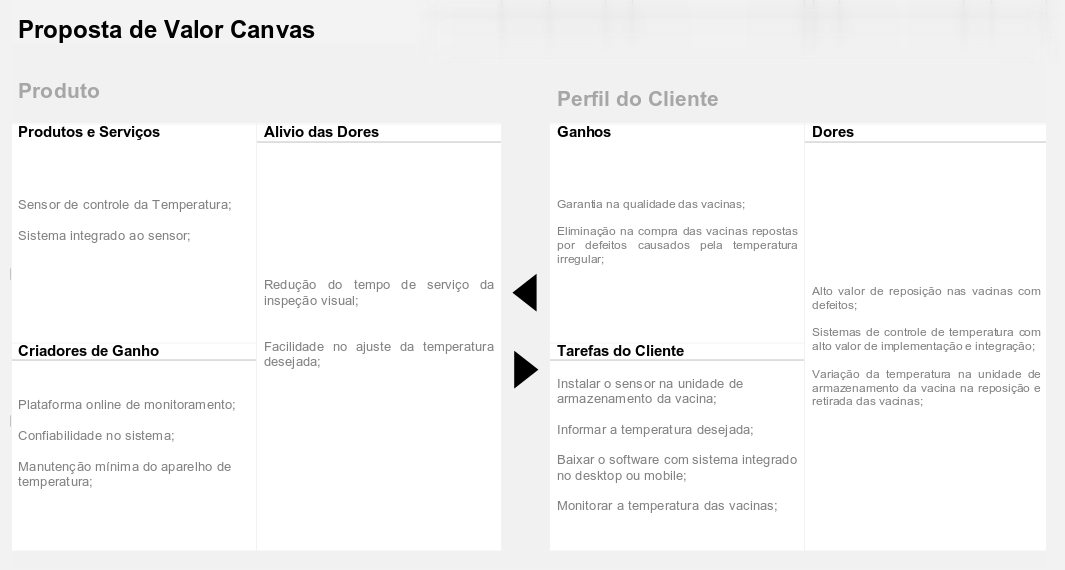
\includegraphics[width=0.9\textwidth]{img/canvas.png}
        \legend{Fonte: Elaborado pelos autores}
        \label{fig:canvas}
    \end{figure}
